\ \\ [-5mm]
   \begin{enumerate}
      \item On obtient les organigrammes suivants : \vspace*{-3mm}
         \begin{multicols}{3}
            \begin{enumerate}
               \item Avec 2 : \\ [2mm]
                  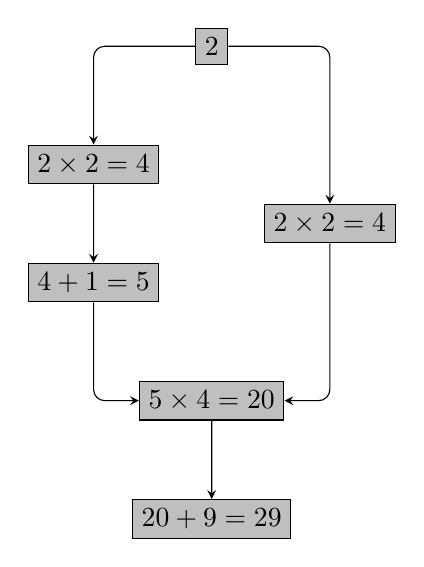
\begin{tikzpicture}[>=stealth,scale=1.5]
                     \node(choix) at (2,5)[rectangle,draw,fill=lightgray] {2};
                     \node(mul) at (1,4)[rectangle,draw,fill=lightgray] {$2\times2 =4$};
                     \node(aj) at (1,3)[rectangle,draw,fill=lightgray] {$4+1 =5$};
                     \node(cal) at (3,3.5)[rectangle,draw,fill=lightgray] {$2\times2 =4$};
                     \node(mul2) at (2,2)[rectangle,draw,fill=lightgray] {$5\times4 =20$};
                     \node(aj2) at (2,1)[rectangle,draw,fill=lightgray] {$20+9 =29$};
                     \draw[->,rounded corners=4pt] (choix) -| (mul);
                     \draw[->,rounded corners=4pt] (choix) -| (cal);
                     \draw[->] (mul) -- (aj);
                     \draw[->,rounded corners=4pt] (cal) |- (mul2);
                     \draw[->,rounded corners=4pt] (aj) |- (mul2);
                    \draw[->] (mul2) -- (aj2);
                  \end{tikzpicture} \\ [2mm]
                  {\blue Avec 2, on obtient 29}.
               \columnbreak
               \item Avec $\dfrac23$ : \\ [2mm]
                  \begin{tikzpicture}[>=stealth,scale=1.5]
                     \node(choix) at (2,5)[rectangle,draw,fill=lightgray] {$\dfrac23$};
                     \node(mul) at (1,4)[rectangle,draw,fill=lightgray] {$2\times\dfrac23 =\dfrac43$};
                     \node(aj) at (1,3)[rectangle,draw,fill=lightgray] {$\dfrac43+1 =\dfrac73$};
                     \node(cal) at (3,3.5)[rectangle,draw,fill=lightgray] {$2\times\dfrac23 =\dfrac43$};
                     \node(mul2) at (2,2)[rectangle,draw,fill=lightgray] {$\dfrac73\times\dfrac43 =\dfrac{28}{9}$};
                     \node(aj2) at (2,1)[rectangle,draw,fill=lightgray] {$\dfrac{28}{9}+9 =\dfrac{109}{9}$};
                     \draw[->,rounded corners=4pt] (choix) -| (mul);
                     \draw[->,rounded corners=4pt] (choix) -| (cal);
                     \draw[->] (mul) -- (aj);
                     \draw[->,rounded corners=4pt] (cal) |- (mul2);
                     \draw[->,rounded corners=4pt] (aj) |- (mul2);
                    \draw[->] (mul2) -- (aj2);
                  \end{tikzpicture} \\ [2mm]
                  {\blue Avec $\dfrac23$, on obtient $\dfrac{109}{9}$}.
               \columnbreak
               \item Avec $x$ : \\ [2mm]
                  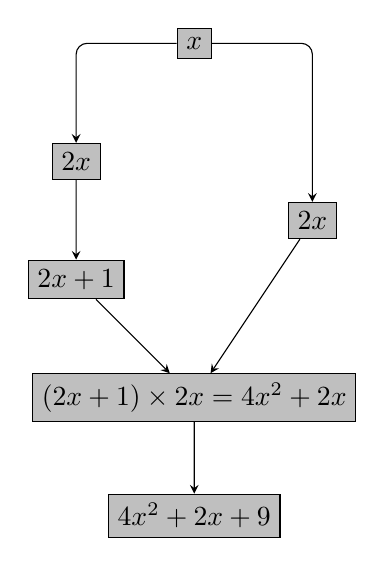
\begin{tikzpicture}[>=stealth,scale=1.5]
                     \node(choix) at (2,5)[rectangle,draw,fill=lightgray] {$x$};
                     \node(mul) at (1,4)[rectangle,draw,fill=lightgray] {$2x$};
                     \node(aj) at (1,3)[rectangle,draw,fill=lightgray] {$2x+1$};
                     \node(cal) at (3,3.5)[rectangle,draw,fill=lightgray] {$2x$};
                     \node(mul2) at (2,2)[rectangle,draw,fill=lightgray] {$(2x+1)\times2x =4x^2+2x$};
                     \node(aj2) at (2,1)[rectangle,draw,fill=lightgray] {$4x^2+2x+9$};
                     \draw[->,rounded corners=4pt] (choix) -| (mul);
                     \draw[->,rounded corners=4pt] (choix) -| (cal);
                     \draw[->] (mul) -- (aj);
                     \draw[->,rounded corners=4pt] (cal) -- (mul2);
                     \draw[->] (aj) -- (mul2);
                    \draw[->] (mul2) -- (aj2);
                  \end{tikzpicture} \\ [2mm]
                  {\blue Avec $x$, on obtient $4x^2+2x+9$}.
            \end{enumerate}
         \end{multicols}
      \setcounter{enumi}{1}
      \item On obtient les résultats suivants : \vspace*{-4mm}
         \begin{multicols}{3}
            \begin{enumerate}
               \item Avec 2 : \\
                  \begin{itemize}
                     \item réponse $\leftarrow$ 2
                     \item résultat $\leftarrow2+3 =5$
                     \item résultat $\leftarrow5\times5 =25$
                     \item {\blue \og le résultat est 25 \fg}.
                  \end{itemize}
                  \columnbreak
               \item Avec 1,5, on obtient : \\
                  \begin{itemize}
                     \item réponse $\leftarrow$ 1,5
                     \item résultat $\leftarrow1,5+3 =4,5$
                     \item résultat $\leftarrow4,5\times4,5 =20,25$
                     \item {\blue \og le résultat est 20,25 \fg}.
                  \end{itemize}
                  \columnbreak
               \item Avec $x$, on obtient : \\
                  \begin{itemize}
                     \item réponse $\leftarrow x$
                     \item résultat $\leftarrow x+3$
                     \item résultat $\leftarrow(x+3)\times(x+3) =x^2+6x+9$
                     \item {\blue \og le résultat est $x^2+6x+9$ \fg}.
                  \end{itemize}
                  \columnbreak
            \end{enumerate}
         \end{multicols}
      \setcounter{enumi}{2}
      \item $4x^2+2x+9 =x^2+6x+9 \iff 3x^2-4x =0$ \\
         \hspace*{4.3cm} $\iff x(3x-4)$ \\
         \hspace*{4.3cm} $\iff x =0 \text{ ou } 3x-4 =0$ \\ [1mm]
         \hspace*{4.3cm} $\iff x =0 \text{ ou } x=\dfrac43$ \\
         {\blue Les programmes donnent le même résultat pour des valeurs égales à 0 ou à $\dfrac43$}.
   \end{enumerate}
